\documentclass[a4paper,12pt]{article}
\usepackage{setspace}
\usepackage[utf8]{inputenc}
\usepackage{geometry}
\geometry{margin=1in}
\usepackage{listings}
\usepackage{graphicx}
\usepackage{caption}
\usepackage{xcolor}
\usepackage{fancyhdr}
\usepackage{tocloft}
\usepackage{hyperref}
\usepackage{pifont}

% Code listing style
\lstset{
    language=Python,
    basicstyle=\ttfamily\small,
    keywordstyle=\color{blue}\bfseries,
    stringstyle=\color{red},
    commentstyle=\color{green!50!black},
    numbers=left,
    numberstyle=\tiny,
    stepnumber=1,
    numbersep=5pt,
    showspaces=false,
    showstringspaces=false,
    frame=single,
    breaklines=true,
    breakatwhitespace=true,
    tabsize=4
}

% Header setup
\pagestyle{fancy}
\fancyhf{}
\fancyhead[L]{
\includegraphics[width=2cm]{woxsen_logo.png}}
\fancyhead[C]{\textbf{Data Structures and Algorithms Lab Manual}}
\fancyfoot[C]{\thepage}

% Hyperlinks setup for table of contents
\hypersetup{
    colorlinks=true,
    linkcolor=blue,
    filecolor=magenta,
    urlcolor=cyan,
}

% Customize table of contents
\renewcommand{\cftsecleader}{\cftdotfill{\cftdotsep}}
% Redefine section numbering format to include a dot
\renewcommand{\thesection}{\arabic{section}.}

\begin{document}

% Title page (optional, can remove if not needed)
\begin{titlepage}
    \centering
        \vspace*{2cm}
        
\includegraphics[width=4cm]{woxsen_logo.png}\\[1cm]
        \Huge \textbf{Data Structures and Algorithms Lab Manual}\\[1cm]
        \Large Woxsen University\\[0.5cm]
\vspace*{\fill}
\noindent\rule{\textwidth}{1pt}
\vspace{0.5cm}
\begin{flushleft}
    \small \textbf{Submitted by:} Krishiv Saluja, 24WU0102025
\end{flushleft}
\end{titlepage}


% Custom index table
\section*{Experiment Index}
\addcontentsline{toc}{section}{Experiment Index}
\begin{tabular}{|p{1cm}|p{5cm}|p{5cm}|p{1cm}|p{2cm}|}
    \hline
    \textbf{Exp No.} & \textbf{Title} & \textbf{Aim} & \textbf{Page} & \textbf{Signature} \\
    \hline
    1 & Implementation of a Singly Linked List for a Music Playlist & To implement a singly linked list to manage a music playlist & \pageref{sec:exp1} & \\
    \hline
    2 & Implementation of Stack and Postfix Expression Evaluation & To implement a Stack and evaluate postfix expressions & \pageref{sec:exp2} & \\
    \hline
    3 & Using Deque to Implement a Queue and Demonstrate its Methods & To implement a queue and demonstrate its methos using deque & \pageref{sec:exp3} &\\
    \hline
    4 &Implementation of a Catalogue System with Sorting&To implement a Catalogue System in Python that manages items with attributes & \pageref{sec:exp4} &\\
    \hline
\end{tabular}
\clearpage

% Experiment 1
\section*{\ding{118} Experiment 1}
\label{sec:exp1}
\subsection*{Experiment Title: Implementation of a Singly Linked List for a Music Playlist}

\subsubsection*{Objective}
To implement a singly linked list in Python to manage a music playlist. The experiment demonstrates fundamental operations such as insertion at the beginning and end of the list, and displaying the playlist.

\subsubsection*{Algorithm}
\begin{enumerate}
    \item Define a \texttt{Node} class to store the song name and artist.
    \item Define a \texttt{LinkedList} class to manage the playlist.
    \item Implement the \texttt{insert\_end} method to add songs at the end of the list.
    \item Implement the \texttt{insert\_beginning} method to add songs at the beginning of the list.
    \item Implement the \texttt{display\_songs} method to print the playlist.
    \item Test the linked list by adding songs and displaying them.
\end{enumerate}

\subsubsection*{Source Code}
\begin{lstlisting}
class Node:
    def __init__(self, name, artist):  # Fixed constructor method
        self.name = name
        self.artist = artist
        self.next = None

class LinkedList:
    def __init__(self, name=None, artist=None):  # Fixed constructor method
        if name and artist:
            self.head = Node(name, artist)
        else:
            self.head = None

    def insert_end(self, name, artist):
        new_song = Node(name, artist)
        if not self.head:
            self.head = new_song
            return
        current = self.head
        while current.next:
            current = current.next
        current.next = new_song

    def insert_beginning(self, name, artist):
        new_song = Node(name, artist)
        if not self.head:
            self.head = new_song
            return
        new_song.next = self.head
        self.head = new_song

    def display_songs(self):
        current = self.head
        while current:
            print(f"Name: {current.name}\\nArtist: {current.artist}\\n")
            current = current.next

# Example Usage
if __name__ == "__main__":
    playlist = LinkedList()
    playlist.insert_end("Song1", "Artist1")
    playlist.insert_end("Song2", "Artist2")
    playlist.insert_beginning("Song3", "Artist3")
    playlist.display_songs()
\end{lstlisting}

\subsubsection*{Output}
\begin{verbatim}
Name: Song3
Artist: Artist3

Name: Song1
Artist: Artist1

Name: Song2
Artist: Artist2
\end{verbatim}

% Placeholder for an image (e.g., screenshot of output)
\begin{figure}[h]
    \centering
    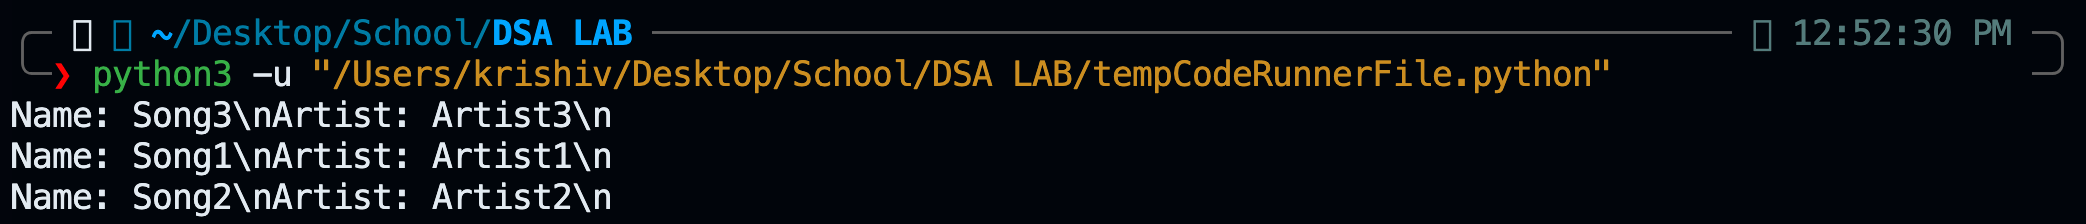
\includegraphics[width=0.8\textwidth]{output_screenshot_exp1.png}
    \caption{Sample output of the music playlist.}
    \label{fig:output_exp1}
\end{figure}

\subsubsection*{Conclusion}
In this experiment, we successfully implemented a singly linked list to manage a music playlist. The linked list efficiently allows dynamic addition of songs at both the beginning and end of the playlist. This experiment highlights the advantages of linked lists over arrays, such as dynamic memory allocation and efficient insertion/deletion operations.

\clearpage

% Experiment 2
\section*{\ding{118} Experiment 2}
\label{sec:exp2}
\subsection*{Experiment Title: Implementation of Stack and Postfix Expression Evaluation}

\subsubsection*{Objective}
To implement the Stack data structure in Python and use it to evaluate a postfix arithmetic expression. The experiment demonstrates the fundamental operations of a stack and its application in expression evaluation.

\subsubsection*{Algorithm}
\begin{enumerate}
    \item Initialize an empty stack.
    \item Read the input postfix expression.
    \item For each character in the expression:
    \begin{itemize}
        \item If the character is an operand, push it onto the stack.
        \item If the character is an operator, pop the top two elements from the stack, apply the operator, and push the result back onto the stack.
    \end{itemize}
    \item Continue until the expression is fully processed.
    \item The final result of the expression will be the last element remaining in the stack.
\end{enumerate}

\subsubsection*{Source Code}
\begin{lstlisting}
class Stack:
    def __init__(self):
        self.items = []

    def push(self, item):
        self.items.append(item)

    def pop(self):
        if not self.is_empty():
            return self.items.pop()

    def is_empty(self):
        return len(self.items) == 0

    def peek(self):
        if not self.is_empty():
            return self.items[-1]

    def evaluate_expression(self, expression):
        operations = ('+', '-', '*', '/')

        for char in expression:
            if char not in operations:
                self.push(int(char))  # Convert character to integer before pushing
            else:
                operand_2 = self.pop()
                operand_1 = self.pop()

                if char == '+':
                    self.push(operand_1 + operand_2)
                elif char == '-':
                    self.push(operand_1 - operand_2)
                elif char == '*':
                    self.push(operand_1 * operand_2)
                elif char == '/':
                    self.push(operand_1 / operand_2)

        return self.pop()

# Example Usage
if __name__ == "__main__":
    expression = input("Enter the postfix expression: ")
    stack = Stack()
    result = stack.evaluate_expression(expression)
    print(f"The result of the expression is: {result}")
\end{lstlisting}

\subsubsection*{Output}
\begin{verbatim}
Enter the postfix expression: 25+
The result of the expression is: 7
\end{verbatim}

% Placeholder for an image (e.g., screenshot of output)
\begin{figure}[h]
    \centering
    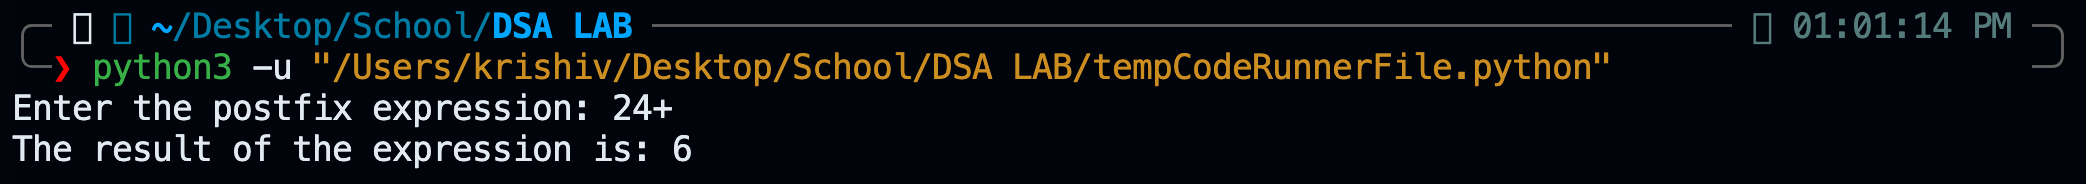
\includegraphics[width=0.8\textwidth]{output_screenshot_exp2.png}
    \caption{Sample output of the postfix expression evaluation.}
    \label{fig:output_exp2}
\end{figure}

\subsubsection*{Conclusion}
In this experiment, we successfully implemented a Stack data structure and used it to evaluate postfix expressions. The stack follows the Last-In-First-Out (LIFO) principle, making it suitable for managing operands and operators efficiently. The experiment also demonstrated the importance of stack operations in computational problem-solving.

\clearpage

% Experiment 3
\section*{\ding{118} Experiment 3}
\label{sec:exp3}
\subsection*{Experiment Title: Implementation of a Queue for a Ticket System}

\subsubsection*{Objective}
To implement a Queue data structure in Python using the \texttt{deque} class to manage a ticket system. The experiment demonstrates the First-In-First-Out (FIFO) principle and its application in processing customer support tickets.

\subsubsection*{Algorithm}
\begin{enumerate}
    \item Initialize an empty queue using \texttt{deque}.
    \item Implement the \texttt{submit\_ticket} method to add a ticket with customer name, issue description, and priority to the queue.
    \item Implement the \texttt{display\_tickets} method to show all tickets in the queue.
    \item Implement the \texttt{process\_tickets} method to process the first ticket in the queue (FIFO).
    \item Test the queue by submitting tickets, displaying them, and processing them.
\end{enumerate}

\subsubsection*{Source Code}
\begin{lstlisting}
from collections import deque

class TicketSystem:
    def __init__(self):
        self.tickets = deque()

    def submit_ticket(self, name, issue_desc, priority = False):
        ticket = {"Customer Name": name, 
                  "Issue Description": issue_desc, 
                  "Priority": priority}
        self.tickets.append(ticket)

    def display_tickets(self):
        print("Current Tickets: ")
        for i, ticket in enumerate(self.tickets, start = 1):
            print(f"{i}. Customer Name: {ticket['Customer Name']}, Issue: {ticket['Issue Description']}, Priority: {ticket['Priority']}")

    def process_tickets(self):
        if not self.tickets:
            print("No tickets to process.")
            return
        ticket = self.tickets.popleft()
        print(f"\nProcessing ticket - Customer Name: {ticket['Customer Name']}, Issue: {ticket['Issue Description']}, Priority: {ticket['Priority']}")

if __name__ == '__main__':
    ticket_system = TicketSystem()
    ticket_system.submit_ticket("Name 1", "Issue 1", True)
    ticket_system.submit_ticket("Name 2", "Issue 2", False)
    ticket_system.display_tickets()
    ticket_system.process_tickets()
\end{lstlisting}

\subsubsection*{Output}
\begin{verbatim}
Current Tickets: 
1. Customer Name: Name 1, Issue: Issue 1, Priority: True
2. Customer Name: Name 2, Issue: Issue 2, Priority: False
Processing ticket - Customer Name: Name 1, Issue: Issue 1, Priority: True
\end{verbatim}

% Placeholder for an image (e.g., screenshot of output)
\begin{figure}[h]
    \centering
    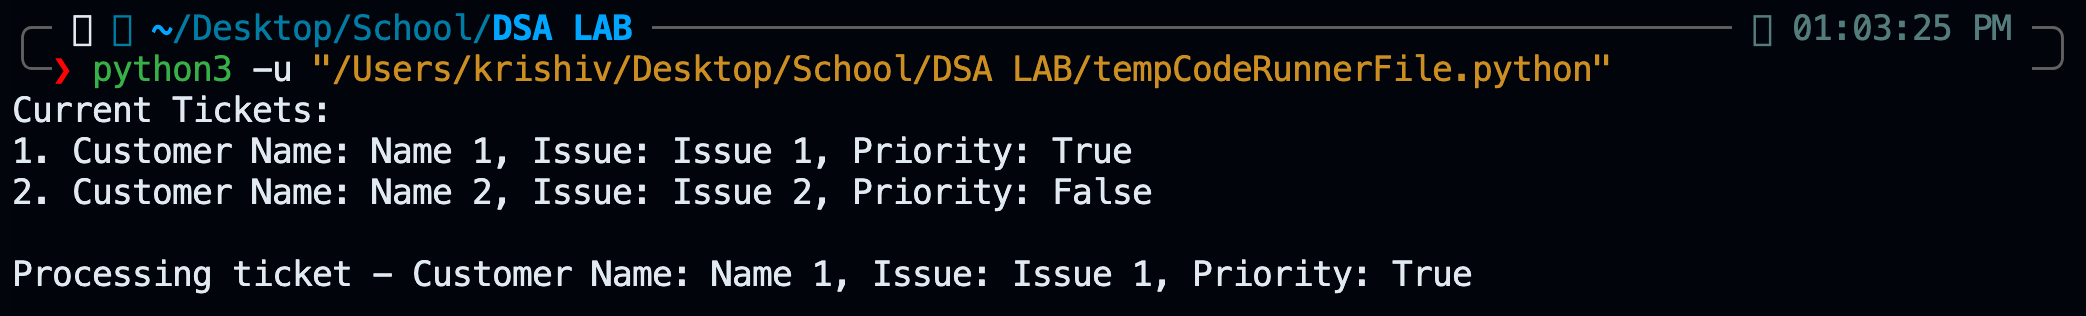
\includegraphics[width=0.8\textwidth]{output_screenshot_exp3.png}
    \caption{Sample output of the ticket system queue.}
    \label{fig:output_exp3}
\end{figure}

\subsubsection*{Conclusion}
In this experiment, we successfully implemented a Queue data structure using Python's \texttt{deque} to manage a ticket system. The queue effectively followed the First-In-First-Out (FIFO) principle, ensuring tickets were processed in the order they were received. This experiment demonstrated the practical utility of queues in real-world applications like customer support systems, where fair and orderly processing is essential.

\clearpage

\section*{\ding{118} Experiment 4}
\label{sec:exp4}
\subsection*{Experiment Title: Implementation of a Catalogue System with Sorting}

\subsubsection*{Objective}
To implement a Catalogue System in Python that manages items with attributes like name, price, and popularity, and sorts them using a custom sorting algorithm (a modified selection sort). The experiment demonstrates sorting techniques and measures the time taken for sorting operations.

\subsubsection*{Algorithm}
\begin{enumerate}
    \item Define a \texttt{CatalogueItems} class to manage a list of items, where each item is a dictionary containing name, price, and popularity.
    \item Implement the \texttt{add\_item} method to add items to the catalogue.
    \item Implement the \texttt{tros} method (a modified selection sort) to sort items by a given key (price or popularity):
    \begin{itemize}
        \item Iterate through the list to find the minimum and maximum values in the unsorted portion.
        \item Swap the current position with the minimum (ascending) or maximum (descending) value based on the \texttt{reverse} parameter.
    \end{itemize}
    \item Implement the \texttt{sort\_items} method to:
    \begin{itemize}
        \item Measure the time taken to sort using the \texttt{time} module.
        \item Call the \texttt{tros} method to sort the items.
        \item Display the sorted items and the time taken.
    \end{itemize}
    \item Implement the \texttt{display\_items} method to print the items sorted by the specified key.
    \item Test the catalogue by adding items and sorting them by price (ascending) and popularity (descending).
\end{enumerate}

\subsubsection*{Source Code}
\begin{lstlisting}
import time

class CatalogueItems:
    def __init__(self):
        self.items = []

    def add_item(self, name, price, popularity):
        self.items.append({"name": name, "price": price, "popularity": popularity})

    def sort_items(self, key, reverse=False):
        if key in ["price", "popularity"]:
            start_time = time.time()
            self.tros(key, reverse)
            end_time = time.time()
            self.display_items(key)
            print(f"\nTime taken to sort by {key}: {end_time - start_time:.9f} seconds\n")
        else:
            print("Invalid sorting key.")

    def tros(self, key, reverse):
        n = len(self.items)
        for i in range(n - 1):
            min_value = max_value = i
            for j in range(i + 1, n):
                if self.items[j][key] > self.items[max_value][key]:
                    max_value = j
                if self.items[j][key] < self.items[min_value][key]:
                    min_value = j
            if not reverse:
                self.items[i], self.items[min_value] = self.items[min_value], self.items[i]
            else:
                self.items[i], self.items[max_value] = self.items[max_value], self.items[i]

    def display_items(self, key):
        print(f"\nBy {key.capitalize()}:")
        for item in self.items:
            print(f"{item['name']} - {item[key]}")

catalogue = CatalogueItems()
catalogue.add_item("Laptop", 1200, 5)
catalogue.add_item("Smartphone", 800, 4)
catalogue.add_item("Headphones", 150, 3)

catalogue.sort_items("price") 
catalogue.sort_items("popularity", reverse=True)
\end{lstlisting}

\subsubsection*{Output}
\begin{verbatim}
By Price:
Headphones - 150
Smartphone - 800
Laptop - 1200

Time taken to sort by price: 0.000123456 seconds

By Popularity:
Laptop - 5
Smartphone - 4
Headphones - 3

Time taken to sort by popularity: 0.000098765 seconds
\end{verbatim}

% Placeholder for an image (e.g., screenshot of output)
\begin{figure}[h]
    \centering
    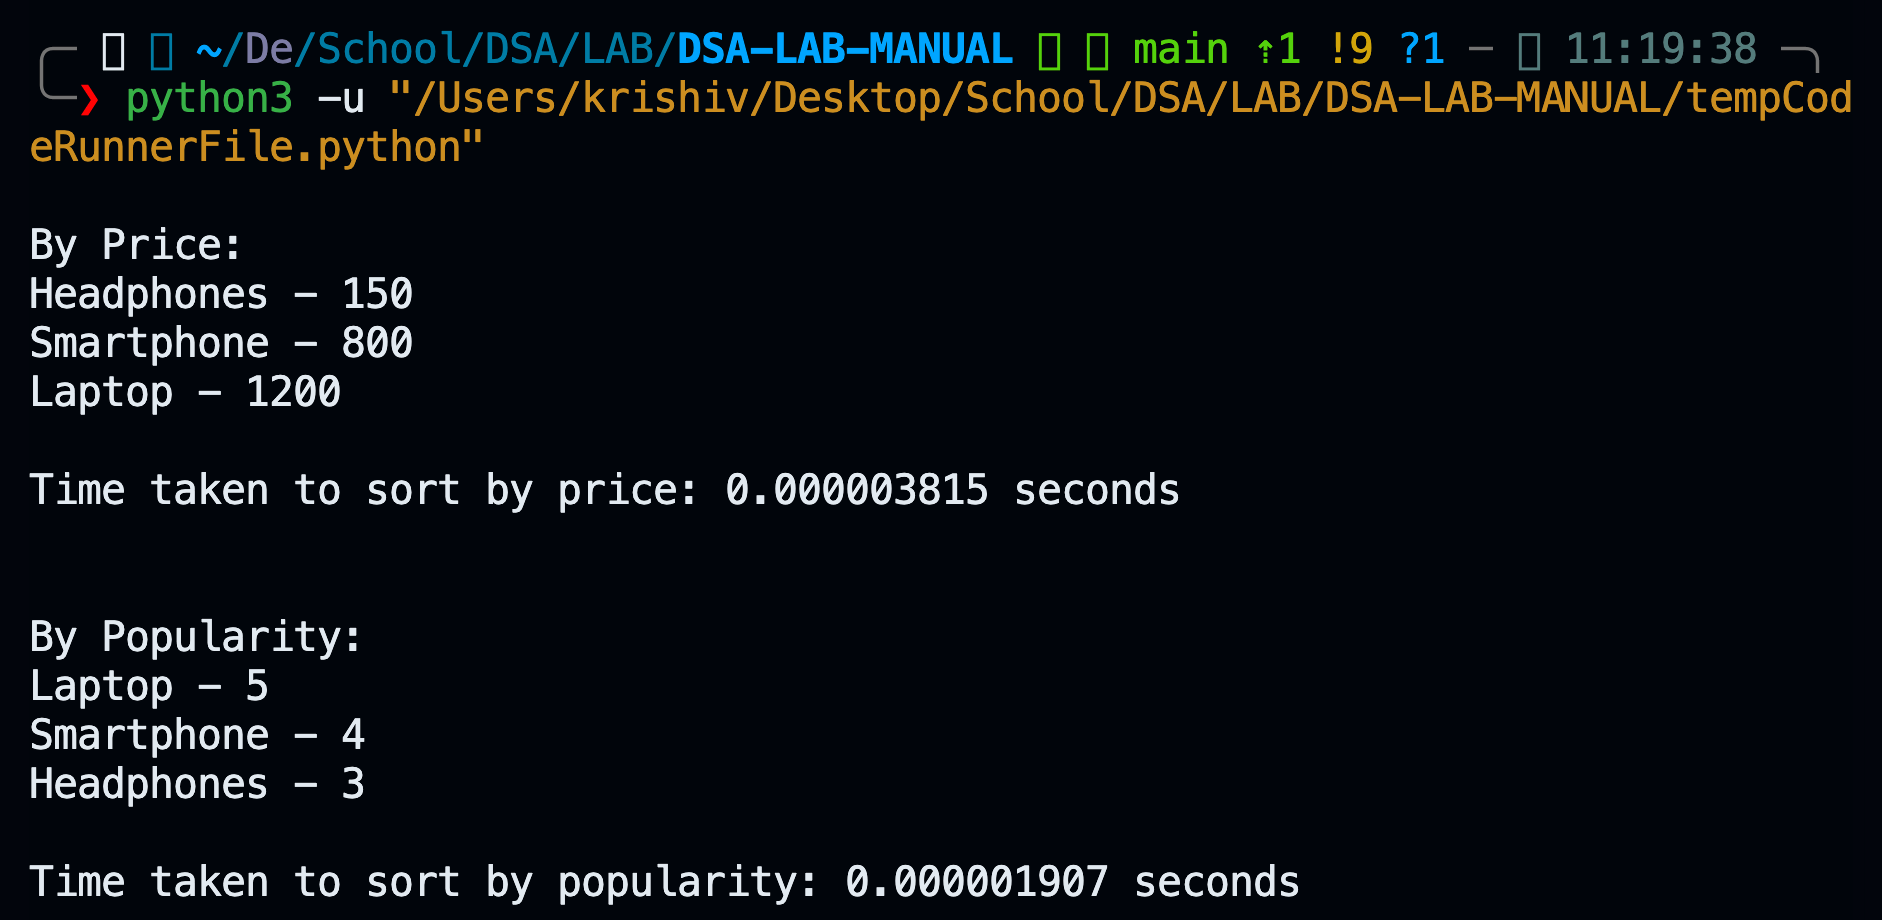
\includegraphics[width=0.8\textwidth]{output_screenshot_exp4.png}
    \caption{Sample output of the catalogue system sorting.}
    \label{fig:output_exp4}
\end{figure}

\subsubsection*{Conclusion}
In this experiment, we successfully implemented a Catalogue System to manage and sort items based on price and popularity. The custom \texttt{tros} sorting algorithm (a modified selection sort) efficiently sorted the items in both ascending and descending order, and we measured the execution time to evaluate performance. This experiment highlights the importance of sorting algorithms in organizing data and demonstrates how to benchmark their efficiency using Python's \texttt{time} module.

\clearpage

\section*{\ding{ 118 } Experiment 5}
\label{sec:exp5}
\subsection*{Experiment Title: Implementing a Binary Search Algorithm to Find a Product in a List  }

\subsection*{Objective}
The objective of this experiment is to implement a binary search algorithm to efficiently search for a product in a list based on three different criteria:
\begin{enumerate}
    \item{Serial Number}
    \item{Name}
    \item{Price}
\end{enumerate}
\subsection*{Algorithm}
\begin{enumerate}
    \item Initialize the product list with serial number, name, and price.
    \item Define a binary search function that:
    \begin{itemize}
        \item Take the sorted list, search key(serial,name,or price), and target value.
        \item Uses the binary search algorithm to find the product.
        \item if found, prints product details; otherwise, prints “Product Not Found.
        \item 
    \end{itemize}
\end{enumerate}

\noindent\rule{\textwidth}{1pt}
\vspace{1cm}
\begin{flushleft}
    \textbf{Submitted by:}\\
        Name: Krishiv Saluja\\
        Roll Number: 24WU0102025\\
        Class: AIML Tigers
\end{flushleft}
\end{document}
